\documentclass[conference]{IEEEtran}

\usepackage{cite}
\usepackage{amsmath,amssymb,amsfonts}
\usepackage{algorithmic}
\usepackage{graphicx}
\usepackage{textcomp}
\usepackage{xcolor}
\usepackage{multirow}
\usepackage{makecell}
\usepackage{float}

\def\BibTeX{{\rm B\kern-.05em{\sc i\kern-.025em b}\kern-.08em
    T\kern-.1667em\lower.7ex\hbox{E}\kern-.125emX}}

\begin{document}

\title{Interpretable Multi-Class Abnormality Classification and Segmentation in Volumetric Chest CT using Dictionary Learning}

\author{
\IEEEauthorblockN{Chamuditha Kekulawala}
\IEEEauthorblockA{
\textit{Department of Electrical and Information Engineering} \\
\textit{Faculty of Engineering, University of Ruhuna} \\
Galle, Sri Lanka \\
kekulawala\_krcs\_e23@engug.ruh.ac.lk
}
\and
\IEEEauthorblockN{Govindu Thejana}
\IEEEauthorblockA{
\textit{Department of Electrical and Information Engineering} \\
\textit{Faculty of Engineering, University of Ruhuna} \\
Galle, Sri Lanka \\
thejana\_bpgl\_e23@engug.ruh.ac.lk
}
\and
\IEEEauthorblockN{Pasan Thilakshana}
\IEEEauthorblockA{
\textit{Department of Electrical and Information Engineering} \\
\textit{Faculty of Engineering, University of Ruhuna} \\
Galle, Sri Lanka \\
thilakshana\_bgpu\_e23@engug.ruh.ac.lk
}
\and
\IEEEauthorblockN{Yasiru Kularathne}
\IEEEauthorblockA{
\textit{Department of Electrical and Information Engineering} \\
\textit{Faculty of Engineering, University of Ruhuna} \\
Galle, Sri Lanka \\
kularathne\_mbyd\_e23@engug.ruh.ac.lk
}
}

\maketitle

\begin{abstract}
Computer Aided Diagnosis (CAD) from volumetric chest Computed Tomography
(CT) requires clinically interpretable methods to support radiological decision-making.
Current State-of-the-Art (SotA) deep learning models often rely on post-hoc explain-
ability methods such as Grad-CAM, that provide approximate localizations and lack
direct traceability to the model\'s decisions. Furthermore, SotA models rarely support
simultaneous multi-class classification and segmentation, leading to a fragmented ap-
proach to diagnosis. This also hinders the ability to benchmark CAD approaches
across multiple dimensions of performance. This study aims to address these chal-
lenges through two contributions: (i) We implement a unified CAD framework that
uses inherently interpretable dictionary learning methods, where detected abnormali-
ties can be represented as a linear combination of “atoms”, allowing predictions to be
projected back to relevant anatomical structures in the CT volume. (ii) We develop
an open-source evaluation framework to benchmark SotA models across three axes:
classification, segmentation and explainability. We use a subset of the ReXGround-
ingCT dataset which provides voxel-level 3D segmentation masks corresponding to
volumetric scans in the CT-RATE dataset. Based on expert radiologist recommen-
dation and dataset availability, pre-processed volumes are patch-sampled for normal
lung parenchyma and two selected pulmonary abnormalities. Using the proposed
benchmarking framework, we evaluate four dictionary learning approaches against
four SotA models and three machine learning baselines, where our best-performing
variant achieved 88\% classification accuracy and 20\% global hit-rate for segmentation,
while providing clinically interpretable voxel-level localizations without the need for
post-hoc explanations. In comparison, the SotA models achieved 97\% classification
accuracy and a 64\% global hit rate.
\end{abstract}

\begin{IEEEkeywords}
Chest CT, Dictionary Learning, Explainability, Segmentation.
\end{IEEEkeywords}

\section{Introduction}
Lung disease remains a leading cause of global morbidity and mortality \cite{murray2022global}. Research
shows that early detection of pulmonary diseases significantly improves patient outcomes.
For this, radiological imaging tools such as Chest X-Ray (CXR) and Computed
Tomography (CT), plays an important role. However, the increasing volume
of such imaging data increases radiologists' workload, leading to delays and potential
errors in diagnosis. This has motivated the development of automated Computer-Aided
Diagnosis (CAD) systems, which use computational algorithms and Artificial
Intelligence (AI) to assist in tasks such as abnormality detection, classification, and
segmentation \cite{doi2007computer}.

\subsection{Motivation}

Developing a unified pipeline for multi-class abnormality classification and grounded
localization addresses two of the most critical imperatives in clinical AI adoption: diagnostic
accuracy and explainability. Specifically, utilizing dense pixel-level segmentation
as the mechanism for localization forces the architecture to provide voxel-level
visual evidence for its diagnostic claims. This ensures that the model is accountable
and its claims are supported by clinical evidence.

Our research mainly focuses on the development of a CAD system using 3 Dimensional (3D)
CT data. While CXR is commonly used as the first imaging test
due to its low cost and low radiation exposure, studies show that their sensitivity to
abnormailities is limited \cite{borakati2020diagnostic}. Comparatively, CT scans produce high resolution cross-sectional
slices that helps detect smaller, early-stage, and subtle lung pathologies that
are frequently missed by standard CXR.

However, CT analysis is complex and time-consuming, requiring radiologists to review
hundreds of slices per scan, which are often inconsistent due to artifacts, anatomical
variations and different scanners/protocols. Furthermore, different anatomical
structures can share identical grayscale values. Telling them apart requires expert
clinical judgment which is often subjective. High sensitivity can lead to detection of
clinically insignificant abnormalities, while visual fatigue can lead to missed findings \cite{mccreadie2009eight}.

\section{Related Work}
To address these challenges, recent research and clinical deployments of AI-based
CAD systems are fundamentally changing how radiologists approach CT analysis. AI
models such as 3D Convolutional Neural Networks (CNNs) and Vision Transformers
(ViTs) have shown to reduce interpretation time, and improve lesion detection sensitivity
compared to traditional manual methods \cite{doi2007computer}. Many of these high performing
models are Deep Learning based, which are criticized for their black box nature, where
their internal reasoning is difficult to interpret [6]. This lack of interpretability is a
significant barrier for clinical adoption, as radiologists require evidence to support a
model's diagnostic claims.

This has motivated the development of explainable AI (XAI) methods such as
Gradient-weighted Class Activation Mapping (Grad-CAM) that helps to visualize
exactly which parts of an image a model focuses on when making a specific prediction.
Such XAI methods are highly valuable for building clinical trust in deep learning
models. However, they often lack the fine-grained, pixel-level precision required to
identify tiny lesions, sometimes highlighting incorrect or confounding features \cite{ennab2025advancing}.
Recent advances in sparse representation models \cite{liyanage2022covid, wesp2026sparse} such as Sparse Autoencoders
and Dictionary Learning have shown to provide inherent interpretability in
medical imaging. This stems from their ability to reconstruct complex, high-dimensional
data as a linear combination of “atoms” or features. This allows the use of efficient
algorithms to easily map the output sparse domain back to the original input feature
space, providing a linear relationship between the model's decision and anatomical
structures. Our work builds on these advances by applying dictionary learning to 3D
Chest CT data for multi-class abnormality classification and grounded localization.

\section{Methodology}
Figure \ref{fig:framework} gives a visual overview of the full framework presented in this study.

\begin{figure}
    \centering
    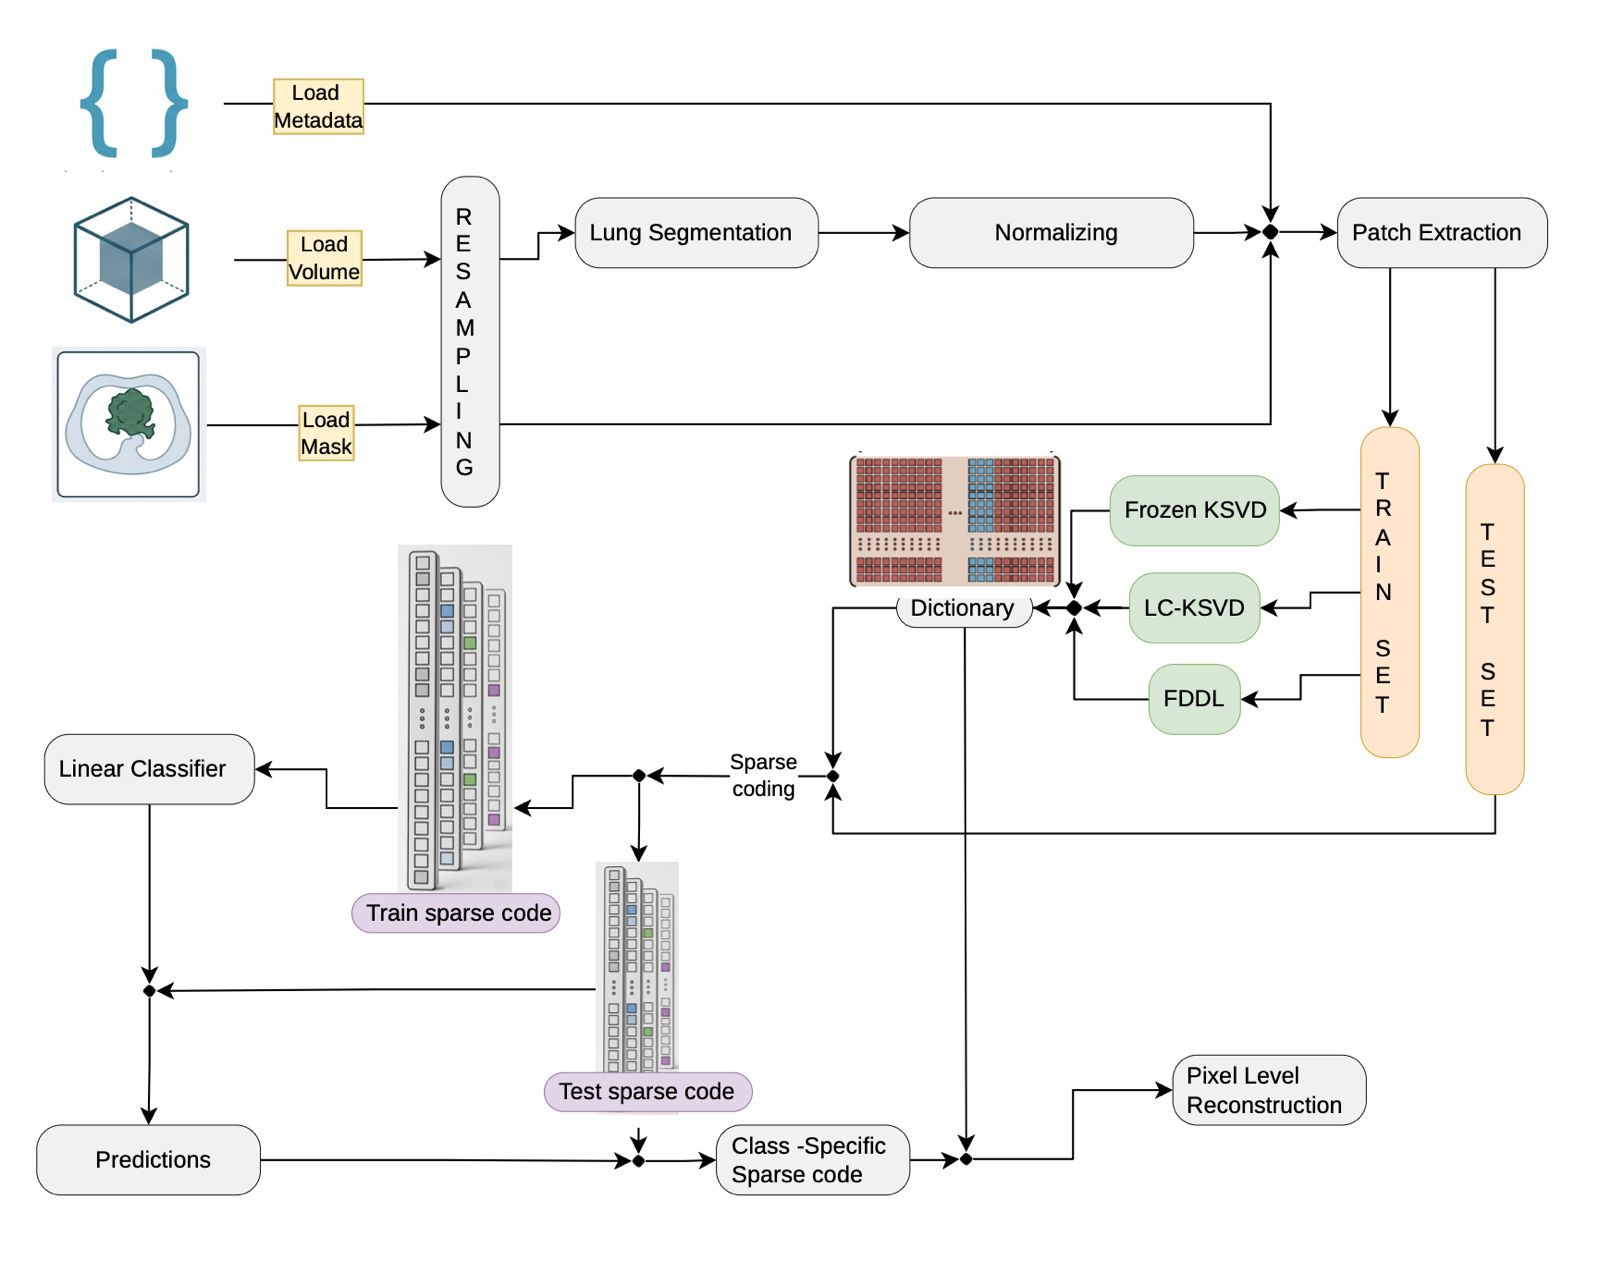
\includegraphics[width=0.5\textwidth]{OverallMethodologyDiagram.jpeg}
    \caption{Overview of the proposed framework for multi-class abnormality classification and segmentation in volumetric chest CT using dictionary learning.}
    \label{fig:framework}
\end{figure}

\subsection{Pre-processing}
We use a subset of the ReXGroundingCT \cite{rajpurkar2024rexgroundingct} dataset which provides voxel-level 3D segmentation masks corresponding
to volumetric scans in the CT-RATE \cite{hamamci2024ctrate} dataset. First, each scan and its corresponding mask is loaded and resampled to
a common voxel spacing, to correct for variable scanner resolutions. We chose the same anisotropic target spacing
used by the pre-processing pipeline of the CT-CLIP \cite{hamamci2024ctclip} model, since it was trained on the volumes from the same
dataset as ours. The target spacing was set to $0.75 \times 0.75 \times 1.5$ mm, in the x, y and z directions respectively. Since chest
CTs naturally often have higher in-plane resolution than axial slice thickness, Setting a 1.5 mm z-spacing respects this
clinical reality while reducing the number of voxels by 50\% compared to isotropic 0.75 mm 3D grids. After resampling,
all volumes and masks were resized to a fixed matrix size of $480 \times 480 \times 240$ voxels across the coronal, sagittal and
axial axes respectively, using center-cropping for oversized volumes or padding for undersized volumes. This again
follows the same approach as the CT-CLIP model, yielding a field of view of $360 \times 360 \times 360$ mm, which spans the
physical volume of a human thorax, ensuring that critical boundaries are not cut off during cropping.

\subsection{Patch Extraction}
Passing the whole volume to the model would include information on bones, soft tissue and background air which
risks letting the model pick up spurious patterns unrelated to lung pathology. Therefore, the lung region had to be
isolated using segmentation. The method that was ultimately adopted is the LungMask library, which uses a U-net
(R231) model [85]. After lung segmentation, the voxel intensities were clipped to a fixed window of $[-1000, 200$] HU.
$1,000$ HU corresponds to air, while the 200 HU upper limit was decided using a histogram analysis of the dataset. For
Normalization, we used Min-Max scaling to $[-1, 1]$ following the same approach used in the CT-CLIP study. Finally,
fixed size patches are extracted for normal lung parenchyma and a set of target abnormalities.
The target abnormalities were decided based on the expert recommendation of a Consultant Radiologist at the
Teaching Hospital, Karapitiya, sufficient representation within the dataset and clinical significance.
The final set of abnormalities was narrowed down to two abnormalities: Ground-Glass Opacity
(GGO), and Nodules/Masses.

A patch size of $12\times12\times6$
is selected by considering the average size of small nodules, the size of the dictionary, loss of context, and
dataset variability. Furthermore, since abnormalities are irregularly shaped, a maximum of 50\% of the voxels in a
patch were allowed to be non-lesion. A similar approach was used for healthy tissue, where a maximum of 50\% of the
voxels in a patch were allowed to be background to avoid patches sampled completely from outside the lung
parenchyma. Each extracted patch is subsequently flattened into a vector representation before being handed to the
dictionary learning algorithms. Figure \ref{fig:patch_extraction} shows the patch extraction pipeline.

\begin{figure}[H]
    \centering
    \includegraphics[width=0.5\textwidth]{patchExtraction.png}
    \caption{Patch extraction pipeline for normal lung parenchyma and target abnormalities.}
    \label{fig:patch_extraction}
\end{figure}

\subsection{Dictionary Learning}
The extracted patches are divided to train and test splits, and four Dictionary Learning algorithms (K-SVD, LC-KSVD,
FDDL and Frozen K-SVD) are trained using the train split. Figure \ref{fig:ksvd_atoms} shows a visualization of the learned atoms from the
K-SVD dictionary. After training the dictionaries, the patches in the train split are re-encoded against each dictionary
to produce a sparse code for each patch. Then, we send each code along with its associated label to a classifier model,
to determine the class of the patch based on its sparse representation. We trained three classifiers for each dictionary
learning algorithm: Logistic Regression, Linear SVM and XGBoost. The performance of each classifier was evaluated on
the same dataset, and the best-performing classifier was selected for each algorithm.

\begin{figure}
    \centering
    \includegraphics[width=0.5\textwidth]{atom_grid_normal_ggo_nodule.png}
    \caption{Visualization of the learned atoms from the K-SVD dictionary.}
    \label{fig:ksvd_atoms}
\end{figure}

The train set is again sparse-coded and a linear classifier trains on these sparse codes and corresponding labels. To
reconstruct the specific voxels in a patch that belong to a particular class, the feature importance of each atom must be
found. For this, we first analyze the sparse codes to find atoms that are class-exclusive. The class selectivity of a sparse
coefficient was calculated by dividing its mean activation for a given class c to its mean activation across all other
classes. From this, the 10 most frequent sparse coefficients are used to reconstruct abnormality in original voxel space.
Figure \ref{fig:reconstruction} shows the final reconstruction of a nodule using the computed sparse coefficients.

\begin{figure}[H]
    \centering
    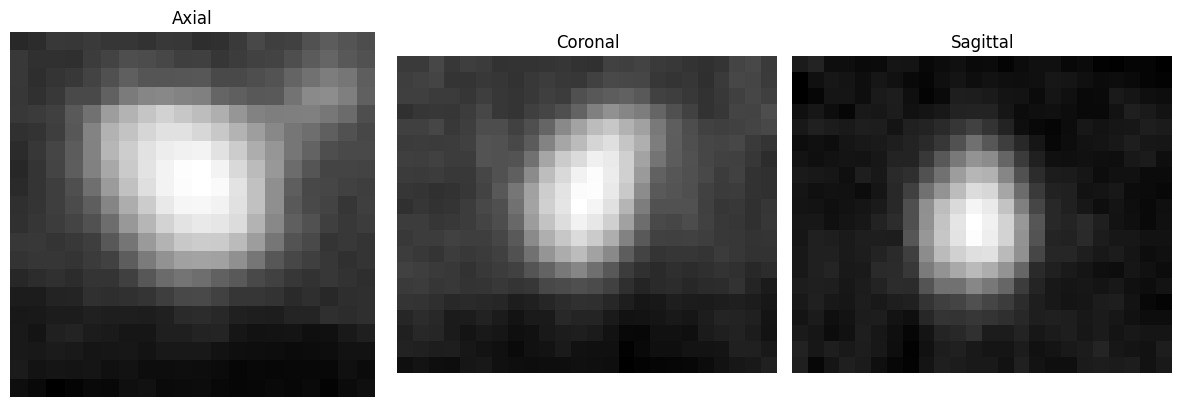
\includegraphics[width=0.5\textwidth]{NoduleReconstruction.jpeg}
    \caption{Final reconstruction of a nodule using computed sparse coefficients.}
    \label{fig:reconstruction}
\end{figure}

\section{Results / Evaluation}
The 11 models compared in this study cover a range of approaches spanning sparse dictionary learning, dense voxel-wise
segmentation, and promptable foundation models. Their outputs at the end of a forward pass range from a
calibrated probability, to a bare class label, to a folder of binary volumes. To design an evaluation framework, all of
these outputs have to be pushed through one common representation. The shared framework consists of three
components: a Runner, Core, and Adapter. The Adapter translates each model's native output into a common case
schema without performing any computations, making it easy to add new models by implementing only this
conversion step. The Core is a model-agnostic library containing consistent metric definitions for classification,
localization, and explainability, operating exclusively on the common schema so that all models are evaluated using
identical calculations. The Runner connects the two by selecting the appropriate Adapter and Core metrics for a given
model and evaluation axis, then producing summary and per-case results.

Table \ref{tab:results-summary} provides a summary of the results across all models and evaluation axes.

\begin{table*}[t]
    \centering
    \caption{Summary of results across all models and evaluation axes.}
    \label{tab:results-summary}
    \renewcommand{\arraystretch}{1.5}
    \begin{tabular}{llcccccccccc}
        \hline
        \textbf{Model Type} & \textbf{Model} &
        \multicolumn{5}{c}{\textbf{Classification}} &
        \multicolumn{3}{c}{\textbf{Segmentation}} &
        \multicolumn{2}{c}{\textbf{Explainability}} \\
        \cline{3-7}
        \cline{8-10}
        \cline{11-12}
        & &
        \textbf{Accuracy} & \textbf{Precision} & \textbf{Recall} &
        \textbf{F1} & \textbf{AU-ROC} &
        \textbf{Dice} & \textbf{Hit Rate} & \textbf{IoU} &
        \textbf{PG Acc.} & \textbf{EIM} \\
        \hline

        \multirow{4}{*}{\makecell{Dictionary\\Learning}}

        & LC-KSVD
        & 0.885 & 0.896 & 0.885 & 0.888 & 0.97
        & 0.010 & 0.200 & 0.005 & -- & -- \\

        & K-SVD
        & 0.664 & 0.653 & 0.630 & 0.631 & 0.72
        & 0.004 & 0.080 & 0.002 & -- & -- \\

        & FDDL
        & 0.766 & 0.759 & 0.724 & 0.737 & 0.83
        & 0.006 & 0.120 & 0.003 & -- & -- \\

        & Frozen DL
        & 0.824 & 0.824 & 0.784 & 0.801 & 0.89
        & 0.008 & 0.160 & 0.004 & -- & -- \\

        \hline

        \multirow{3}{*}{\makecell{Machine\\Learning}}
        & Linear SVM
        & 0.592 & 0.580 & 0.580 & 0.580 & 0.65
        & -- & -- & -- & -- & -- \\

        & Log. Regression
        & 0.554 & 0.539 & 0.540 & 0.539 & 0.62
        & -- & -- & -- & -- & -- \\

        & XGBoost
        & 0.524 & 0.510 & 0.509 & 0.510 & 0.57
        & -- & -- & -- & -- & -- \\

        \hline

        \multirow{4}{*}{\makecell{Deep\\Learning}}
        & CT-CLIP
        & 0.600 & 0.594 & 0.587 & 0.590 & 0.68
        & -- & -- & -- & -- & -- \\

        & Merlin
        & 0.950 & 0.950 & 0.948 & 0.949 & 0.99
        & 0.77 & 0.86 & 0.63 & 0.93 & 0.84 \\

        & BiomedParse
        & -- & -- & -- & -- & --
        & 0.06 & 0.09 & 0.03 & 0.67 & 0.81 \\

        & nnU-Net
        & -- & -- & -- & -- & --
        & 0.10 & 0.14 & 0.05 & -- & -- \\

        \hline
    \end{tabular}
\end{table*}

\section{Discussion}
Four dictionary learning methods (K-SVD, LC-KSVD2, FDDL, Frozen Dictionary Learning) were implemented in an
open-source package and evaluated, alongside three ML baselines and four SotA deep learning models, using a
shared, model-agnostic evaluation framework.

LC-KSVD outperformed all other dictionary learning models, reaching 88.5\% patch accuracy. Patch-level accuracy did not
transfer to whole-volume localisation for any dictionary learning method, a gap
driven by the extreme size imbalance between lesions and full volumes rather than by the sparse codes
themselves. Dictionary learning trails SotA deep learning substantially on raw performance, confirming a
interpretability-performance trade-off.

The study only covers two of five radiologist-recommended abnormalities and excludes the ambiguous
atelectasis/consolidation category. The fixed $12\times12\times6$ patch size discarded most candidate nodule
patches and biased the retained set toward larger masses.

The results of this study should be read alongside several limitations. The evaluation scope was narrowed to
two of the five abnormalities originally recommended by the consulting radiologist.
The qualitative evaluation reflects the judgement of a single radiologist without a second reader, and suggested
that some ground-truth masks may themselves be imperfect references, meaning the absolute Dice and hit-rate
figures reported throughout this thesis are plausibly a lower bound on true clinical usefulness rather than a precise
estimate of it.

The radiologist judged several ReXGroundingCT ground-truth masks to be over-inclusive, with the model's own
predictions more tightly localised to the true abnormality. If this
generalises, reported Dice/IoU figures throughout this chapter are a lower bound on true localisation quality,
not an accurate estimate of it. This does not change relative rankings between models, since all are scored
against the same annotations, but it is a material caveat on any absolute claim.

\section{Conclusion}
This study addressed two gaps in dictionary learning for CT-based CAD: the lack of a framework unifying
multi-class classification and voxel-level localisation, and the lack of any study benchmarking dictionary
learning against deep learning across classification, localisation, and explainability simultaneously. 

Priority directions include, spatially-aware post-processing to close the patch-to-volume localisation gap; extending
to the remaining radiologist-recommended abnormalities, domain-specific hyperparameter tuning
against a held-out validation set, and a second independent radiologist review with inter-rater reliability
reporting.

Dictionary learning is not yet competitive with state-of-the-art deep learning on raw classification or
localisation accuracy for pulmonary abnormality detection, but the interpretability it offers is qualitatively
different from, and more reliable than, Grad-CAM's post-hoc
explanations on a leading vision-language model. A CAD system built on class-attributable atoms can show
exactly which learned pattern drove a prediction and where it is located.
The open-source benchmarking framework developed here is intended to make
that trade-off measurable for future work.

\bibliographystyle{IEEEtran}
\bibliography{references}

\end{document}
